	Αφού τα όρια της $v_2$ ισούνται με  $±\(V_D+V_Z\)$, προκύπτει ότι $v_{2,\max}$ = 8.3V και $v_{2,\min}$ = -8.3V.
	Από την σχέση $\displaystyle{v_{\mathrm{out}}=v_2\cdot\(\sfrac{R_f}{R_1}\)}$ προκύπτει ότι $v_{\mathrm{out},\max}$ = 5.83V και $v_{\mathrm{out},\min} = -5.83\unit{\volt}$.
	Τέλος από τα $v_2$ και $v_{\mathrm{out}}$ προκύπτει $v_{1,\max}$ = 6.85V και $v_{1,\min} = -6.85\unit{\volt}$.
	Από τη σχέση \eqref{eq:ask1_freq} προκύπτει ότι η περίοδος των κυματομορφών είναι $T = 528\unit{\micro\second}$.
	Με βάση τα παραπάνω μπορούμε να σχεδιάσουμε τις κυματομορφές σε βαθμονομημένους άξονες.

\begin{plot_fig}[H]
	\begin{center}
		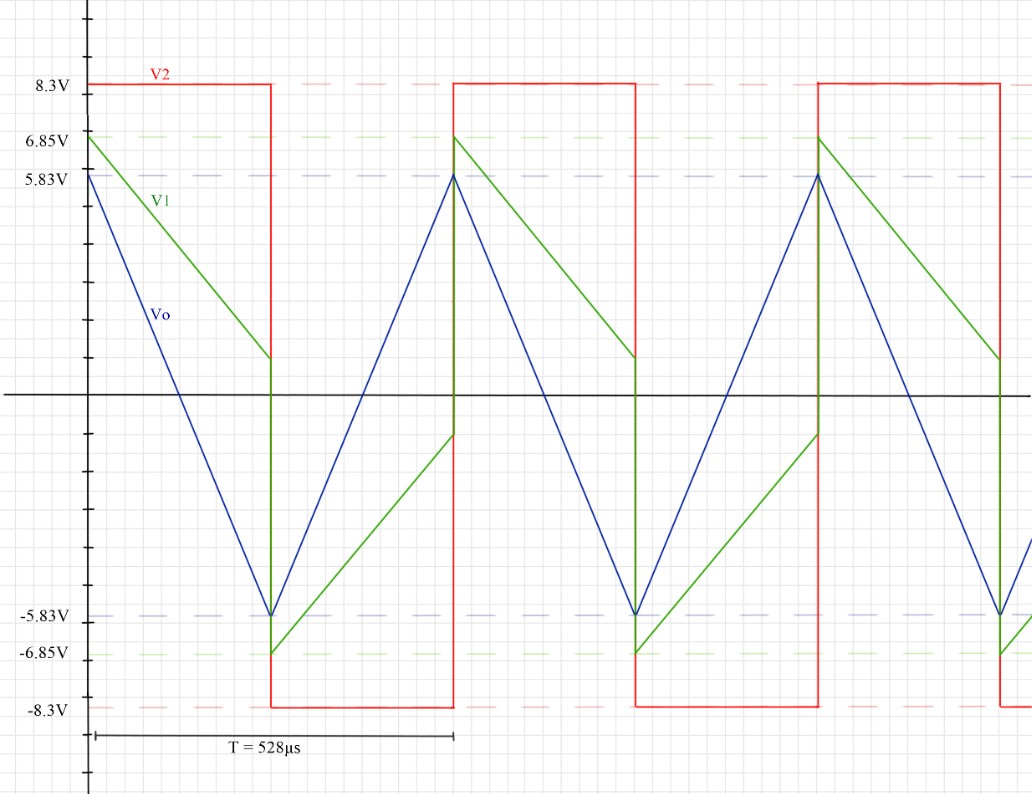
\includegraphics[width=8cm]{charts/1.2_diagram}
		\caption{Κυματομορφές $v_2$, $v_1$ και $v_{\mathrm{out}}$}
		\label{plot:ask1:q2_1}
	\end{center}
\end{plot_fig}
\vspace*{-0.5cm}
Η $v_1$ είναι το άθροισμα του τετραγωνικού παλμού $v_2$ και του τριγωνικού παλμού $v_{\mathrm{out}}$.